%% 信学技報（IEICE Technical Report）原稿 骨組み — 締切 2026-09-14
%% クラス: ieicej.cls v3.4a（同ディレクトリ。配布元 ieice.org 研究会ページ ieicej3.4a.zip）
%% コンパイル: Overleaf で Compiler=uplatex（LuaLaTeX 非対応）。文献は sieicej.bst。
%% 表は tables/*.tex を \input（make_tables_20260915.py が JSON から生成。手打ち禁止）。
%% 注意: 表1（9列）・主表（7列）は段幅（約 240pt）を超える見込み（レビュー 9/7）。対処は table* 化か行ラベルの短縮か 計 列の削除。
%% 原稿枚数は 6 枚以下（原稿執筆依頼の記載、9/10 確認）。LaTeX レビューの見積りは表 5 つ・長いあらましで約 5.9 頁 → 優劣表・係数表を本文に圧縮し、あらましを短縮済み。Overleaf で 5.5 頁以下なら 2 表を戻してよい
%% 本文は 2026-09-10 に paper-manuscript skill §3（2×2 の順位予測 → CL の差 → 仮説 → 数値予測の限界）に沿って初稿を書いた。
%% 「TODO(決定B-n)」は daily_reports/0907.md §B のチェックリスト番号に対応するユーザー決定事項。
%% 「%% [7/27予稿]」以下のコメント行は yokou_20260727.tex からの再利用候補（数値はフェーズ1/2＝DeepGaitV2特徴のもの。X2 の値ではない）。
\documentclass[technicalreport]{ieicej}
\usepackage[dvipdfmx]{graphicx}
\usepackage[fleqn]{amsmath}
\usepackage{newtxtext}% 英数字フォントの設定を変更しないでください
\usepackage[varg]{newtxmath}% 英数字フォントの設定を変更しないでください

\tecrepyear{2026}
%% 決定B-2（9/10 ユーザー指定）: 和文・英文タイトル確定。副題は主題に ft（再学習）が含まれるため付けない
\jtitle{深層特徴空間のデータ特性に基づく歩容認証における学習・再学習データの有効性評価}
%\jsubtitle{}
\etitle{Evaluation of Training and Fine-Tuning Data Effectiveness for Gait Recognition Based on Data Characteristics in Deep Feature Spaces}
%\esubtitle{}
%% 決定B-3（9/10 ユーザー指定）: 著者は 計良 夏輝・村松 大吾（同一所属 Seikei）。連絡先メールは発表者のみ。村松先生の英語表記は要確認
\authorlist{%
 \authorentry[us234030@cc.seikei.ac.jp]{計良 夏輝}{Natsuki KERA}{Seikei}
 \authorentry[]{村松 大吾}{Daigo MURAMATSU}{Seikei}
}
\affiliate[Seikei]{成蹊大学理工学部\hskip1zw
  〒180--8633 東京都武蔵野市吉祥寺北町3--3--1}
 {Faculty of Science and Technology, Seikei University\hskip1em
  3--3--1 Kichijoji-kitamachi, Musashino-shi, Tokyo, 180--8633 Japan}

\begin{document}
\begin{jabstract}
深層特徴空間のデータ特性指標から学習データの有効性を学習前に推定する枠組みを，事前学習済みモデルの再学習による精度改善の予測へ拡張する．特徴抽出器として汎用画像モデルと歩容認証モデルのそれぞれを用い，ゼロからの学習と再学習の両方に対する予測性能を比較する．CASIA-B を分割した特性の異なる複数の学習サブセットを用いた実験結果を報告する．
\end{jabstract}
\begin{jkeyword}
深層学習，学習データ，データ特性，歩容認証，ファインチューニング，認証精度
\end{jkeyword}
\begin{eabstract}
We extend a framework that estimates the effectiveness of training data before training, from data characteristics measured in deep feature spaces, to the prediction of accuracy improvement obtained by fine-tuning a pre-trained model. Using a general-purpose image model and a gait recognition model as feature extractors, we compare the prediction performance for training from scratch and for fine-tuning. We report experimental results on multiple training subsets with different characteristics constructed from CASIA-B.
\end{eabstract}
\begin{ekeyword}
Deep Learning, Training Data, Data Characteristics, Gait Recognition, Fine-tuning, Recognition Accuracy
\end{ekeyword}
\maketitle

%% =====================================================================
\section{まえがき}
歩容認証は歩き方の特徴から個人を識別する技術であり，遠距離かつ非接触で本人の協力なしに識別できるため社会的な需要が高い．近年は深層学習により精度が向上したが，大規模な学習データを要する．歩容データの収集には被験者の撮影協力と同意が不可欠で，多様な服装・所持品・視野角を網羅するとコストが急増する．

課題は，どのようなデータを集めれば精度が上がるのかが事前には分からない点である．学習して初めて価値が分かるが，深層モデルの学習には時間と計算資源を要し，網羅的に試すことは現実的でない．
この課題に対し中村ら\cite{Nakamura_IEICE}は，学習データの特性を深層特徴空間上の統計量として定量化し，対象データで学習を行わずに認証精度を予測する枠組みを提案した．ただし中村らの枠組みには二つの制約がある．第一に，特徴抽出器が歩容に特化しない汎用の画像認識モデルに限られている．第二に，予測対象がゼロから学習する設定（以下スクラッチ学習）の精度に限られている．実務では大規模データで事前学習したモデルをファインチューニングする使い方が主流であり，この設定で学習前の予測が成立するかは未検証である．

そこで本稿では，特徴空間と予測対象の両方を拡張する．特徴空間には，汎用画像モデル（InceptionV3，DINOv2）に加えて歩容認証モデル DeepGaitV2\cite{Fan_DeepGaitV2}を用いる．予測対象には，スクラッチ学習後の精度に加えて，別データセット SUSTech1K\cite{Shen_LidarGait}で事前学習したモデルをファインチューニングした後の精度を用いる．汎用画像特徴$\times$スクラッチ学習の組は中村らの設定に対応し，残る 3 通りが本稿で新規に検証する組合せである．ただしスクラッチ学習精度とファインチューニング後精度の順位は高く相関するため（5.\,1 節），本稿の関心は予測の成否に加えて，どの特徴空間がどの条件で有効かにある．CASIA-B\cite{Yu_CASIAB}の 13 サブセットを用い，4 通りでの順位相関，特徴空間による得意条件の違い，数値予測の破綻を報告する．

%% =====================================================================
\section{関連研究}
\subsection{Fr\'echet Inception Distance}
Fr\'echet Inception Distance（FID）\cite{Heusel_FID}は，画像集合を ImageNet\cite{Russakovsky_ImageNet}で学習した InceptionV3 の特徴空間に写像し，2 つの集合の特徴分布をガウス分布で近似したときの Fr\'echet 距離である．FID は特徴抽出器の選択に依存し，Cetin ら\cite{Cetin_FacialFD}は顔画像に特化した特徴抽出器が分布距離と近傍関係の評価に与える利点と限界を報告している．本稿はこの議論を精度予測という用途で検証する位置づけにある．

\subsection{データ特性に基づく学習データの有効性評価}
中村ら\cite{Nakamura_IEICE}は，CASIA-B から特性の異なる 13 サブセットを構成し，各サブセットの学習画像を InceptionV3 と DINOv2 の特徴空間に写像して，平均クラス内分散，平均類似クラス間距離，平均クラス間距離，Train-Test データ間分布距離の 4 指標を計測した．これら深層特徴の指標と，原画像で計算した平均クラス内分散（中村らの MSD-raw）から，スクラッチ学習後の認証精度を leave-one-dataset-out（LODO）のリッジ回帰で予測し，Spearman 順位相関（以下 $\rho$）0.835 を報告している．2 サブセットの優劣を 3 クラス（優・劣・同等）に分類する優劣判定も行っている．本稿はこの枠組みを踏襲し，予測対象と特徴空間を拡張する．説明変数は，各特徴空間の指標のみで比較するため生画素空間の指標である MSD-raw を用いず，どの特徴空間にも依らない学習人数 $P$（15〜75 名）を共通の説明変数 $\log P$ として与える点が異なる．なお中村らの認証精度は通常歩行（NM），鞄所持（BG），コート着用（CL）の各条件の Rank-1（1 位正解率）の単純平均であり，本稿の定義（4.\,1 節）とは異なるため数値は直接比較しない．

\subsection{歩容認証モデルと事前学習}
DeepGaitV2\cite{Fan_DeepGaitV2}はシルエット系列から歩容特徴を抽出する深層モデルで，屋内外の複数データセットで高い精度を示している．SUSTech1K\cite{Shen_LidarGait}は屋外で収集された大規模歩容データセットで，衣服・所持品・視野角などの多様な条件を含む．本稿では SUSTech1K で事前学習した DeepGaitV2 を，指標を計測する特徴抽出器とファインチューニングの初期値の両方に用いる．

%% =====================================================================
\section{データ特性評価指標}
\subsection{概要}
学習データセットの画像を深層モデルで特徴ベクトルに変換し，クラス（人物）ラベルを用いて次の 4 指標を計測する．（1）平均クラス内分散，（2）平均類似クラス間距離，（3）平均クラス間距離，（4）Train-Test データ間分布距離．平均類似クラス間距離は $k=1$ と $k=5$ の 2 変数として用いるため深層特徴の指標は 5 変数となり，これに $\log P$ を加えた 6 変数を 1 つの特徴空間あたりの説明変数とする．本稿の拡張点は特徴抽出器に DeepGaitV2 を加えたことにある（平均クラス内分散の集計は特徴空間で異なる，3.\,3 節）．

\subsection{特徴抽出}
汎用画像特徴には，ImageNet で学習した InceptionV3\cite{Szegedy_InceptionV3}の特徴と，自己教師あり学習で得られた DINOv2\cite{Oquab_DINOv2}の特徴を用いる．歩容特化特徴には SUSTech1K で事前学習した DeepGaitV2 を用い，出力 $256\times16$ を 1 次元に並べた 4096 次元とした．いずれの特徴抽出器も CASIA-B を学習しておらず，全サブセット共通の抽出器を用いることで指標値をサブセット間で比較可能にしている．InceptionV3 と DINOv2 の指標は画像を，DeepGaitV2 の指標は系列（1 人物・1 条件・1 視野角の連続したシルエット）を単位として計算するため，指標値そのものは特徴空間間で比較せず，各特徴空間内でのサブセット間の変動のみを回帰に用いる．

\subsection{平均クラス内分散}
クラス $s$ に属する特徴ベクトルを $\boldsymbol{x}_i^{s}\,(i=1,\dots,N_s)$，その平均を $\boldsymbol{\mu}_s$ とすると，平均クラス内分散（以下 MSD）$\sigma^2$ は
\begin{align}
\sigma^2 = \frac{1}{M}\sum_{s=1}^{M}\frac{1}{N_s}\sum_{i=1}^{N_s}\|\boldsymbol{x}_i^{s}-\boldsymbol{\mu}_s\|^2
\label{eq:MSD}
\end{align}
で定義される．ここで $M$ はクラス数である．DeepGaitV2 特徴では系列を単位として式\eqref{eq:MSD}のとおり人物ごとに計算した．一方，InceptionV3 と DINOv2 の値は中村らの実装を引き継いでおり，人物を区別せずサブセット内の全画像の特徴平均からの二乗偏差を画像と特徴次元で平均した値である．両者は集計の単位（系列／画像）と範囲（人物ごと／全体）が異なり，値の直接比較はできない．

\subsection{平均類似クラス間距離}
各特徴ベクトルについて，異なる人物に属する特徴ベクトルから近い順に $k$ 個を選んでその距離を平均し，全特徴ベクトルで平均したものを k-NN 距離とする．近傍の $k$ 個は同じ人物から複数選ばれてもよい．本稿では $k=1$ と $k=5$ を用いる（以下それぞれ 1NN，kNN）．値が小さいほど別人物の似たデータがあり識別が難しい．

\subsection{平均クラス間距離，Train-Test データ間分布距離}
平均クラス間距離（以下 pairFID）は，2 つのクラスの特徴分布をガウス分布で近似した FID\cite{Heusel_FID} を全クラス対について計算し平均したものである．Train-Test データ間分布距離（以下 FID$_{\mathrm{tt}}$）は，学習データ全体とテストデータ全体の間の FID である．FID$_{\mathrm{tt}}$ の参照集合には，評価対象の分布を表すラベル不要の集合としてテストデータ（4.\,1 節，49 名）の特徴を用いる．したがって FID$_{\mathrm{tt}}$ の計測にはテスト画像は必要だが，そのラベルも認証モデルの学習も必要としない．

%% =====================================================================
\section{評価実験}
%% 段抜き表（table*）はページ上部にしか置けないため、参照より前の位置で読み込む（LaTeX レビュー 9/10）
%% 自動生成: make_tables_20260915.py（手で編集しない）
\begin{table*}[tb]
\caption{CASIA-B サブセットの構成（学習系列数・人数）と精度（\%，4.\,1 節の定義）．$\Delta$ はファインチューニング後 $-$ スクラッチ学習（pt）．}
\label{tab:subsets}
\begin{center}
\begin{tabular}{l|rrrr|r|rrr}
\Hline
サブセット & NM & BG & CL & 計 & 人数 & scratch & ft & $\Delta$ \\
\hline
default & 984 & 328 & 328 & 1640 & 15 & 69.00 & 78.37 & $+9.37$ \\
nm2 & 1642 & 0 & 0 & 1642 & 75 & 81.17 & 84.03 & $+2.86$ \\
bg2 & 0 & 1642 & 0 & 1642 & 75 & 80.98 & 85.38 & $+4.40$ \\
cl2 & 0 & 0 & 1642 & 1642 & 75 & 73.88 & 83.14 & $+9.26$ \\
nm1-bg1 & 820 & 821 & 0 & 1641 & 75 & 85.35 & 87.86 & $+2.50$ \\
nm1-cl1 & 820 & 0 & 823 & 1643 & 75 & 88.71 & 91.67 & $+2.96$ \\
bg1-cl1 & 0 & 821 & 823 & 1644 & 75 & 87.25 & 90.61 & $+3.36$ \\
000-180 & 893 & 297 & 298 & 1488 & 75 & 40.02 & 57.11 & $+17.09$ \\
000-090 & 894 & 298 & 298 & 1490 & 75 & 59.71 & 79.28 & $+19.58$ \\
090-180 & 899 & 299 & 300 & 1498 & 75 & 59.16 & 77.46 & $+18.30$ \\
nm1-bg1-cl1 & 549 & 546 & 548 & 1643 & 50 & 85.09 & 89.74 & $+4.65$ \\
nm2-bg2-cl2 & 548 & 548 & 548 & 1644 & 25 & 73.69 & 83.07 & $+9.38$ \\
nm6 & 1644 & 0 & 0 & 1644 & 25 & 73.07 & 79.26 & $+6.19$ \\
\Hline
\end{tabular}
\end{center}
\end{table*}

%% 自動生成: make_tables_20260915.py（手で編集しない）
\begin{table*}[tb]
\caption{学習前予測の性能（13 サブセットの LODO）．$\rho$ は Spearman 順位相関，MAE の単位は pt，$p$ は並べ替え検定（1,000 回，片側，$p=(r+1)/(N+1)$．$<$0.001 は超過 0 回）．$\dagger$ はスクラッチ学習について事後に追加した検定．}
\label{tab:main}
\begin{center}
\begin{tabular}{l|ccc|ccc}
\Hline
 & \multicolumn{3}{c|}{スクラッチ} & \multicolumn{3}{c}{ファインチューニング} \\
特徴空間 & $\rho$ & MAE & $p$ & $\rho$ & MAE & $p$ \\
\hline
Inception（6 変数） & 0.879 & 7.18 & $<$0.001$^{\dagger}$ & 0.896 & 1.84 & $<$0.001 \\
DINOv2（6 変数） & 0.808 & 10.39 & $<$0.001$^{\dagger}$ & 0.830 & 3.80 & $<$0.001 \\
Inception+DINOv2（11 変数） & 0.857 & 9.63 & $<$0.001$^{\dagger}$ & 0.885 & 3.92 & $<$0.001 \\
DeepGaitV2（6 変数） & 0.808 & 6.41 & 0.003$^{\dagger}$ & 0.742 & 4.38 & 0.004 \\
\Hline
\end{tabular}
\end{center}
\end{table*}

\subsection{歩容データセット}
CASIA-B\cite{Yu_CASIAB}は 124 名の歩容シルエット系列からなり，各人物について NM 6 系列，BG 2 系列，CL 2 系列が 11 視野角で撮影されている．学習候補を 001--075 の 75 名，テストを 076--124 の 49 名とし，テストは全サブセットで共通である．評価は CASIA-B の標準プロトコルに従い，各人物の NM 第 1〜4 系列をギャラリー，NM 第 5〜6 系列，BG，CL の各 2 系列をプローブとして，同一視野角の組を除外した Rank-1 を条件別に求める（プローブ数は NM 1078，BG 1076，CL 1078）．認証精度は NM/BG/CL 各条件の Rank-1 を固定重み 0.6，0.2，0.2 で平均した値（以下，精度）を用いる．この重みは CASIA-B の各人物の系列構成比（NM 6，BG 2，CL 2）に基づく．条件別の分析では各条件の Rank-1 をそのまま用いる．

\subsection{特性の異なるサブセット}
表\ref{tab:subsets}に，中村ら\cite{Nakamura_IEICE}と同じ設計で構成した 13 サブセットを示す．学習系列数を約 1640 に揃えたうえで，条件（NM/BG/CL の組合せ），人数，視野角のいずれかを削っている．サブセット名は 1 人あたりの系列構成（例えば nm2 は NM 2 系列，nm1-bg1-cl1 は各条件 1 系列，いずれも 11 視野角）または用いる 2 つの視野角の組（例えば 000-180 は $0^\circ$ と $180^\circ$ のみ）を表し，default は 15 名の全系列からなる基準構成である（系列数を揃えるため 1 人あたりの系列が多い構成ほど人数は少ない）．視野角を制限した 3 サブセット（000-180，000-090，090-180）は 75 名分の系列を用いており，系列数が他と異なる．表には 4.\,3 節の設定によるスクラッチ学習（表中 scratch）とファインチューニング（表中 ft）の精度，およびその差 $\Delta$（ファインチューニング後 $-$ スクラッチ学習，単位はパーセントポイント，以下 pt）を併記した．
スクラッチ学習精度は全 13 サブセットについて，中村らの実験で得られた条件別 Rank-1（論文には単純平均のみ掲載）を用いた\footnote{6 サブセットは中村らの学習済みモデルの再評価で同じ値を得た．残る 6 サブセットは本稿で再学習し，5 サブセットは 0.1\,pt 以内，090-180 は 1.7\,pt 以内で一致した．bg1-cl1 は未照合である．}．ファインチューニングは全サブセットについて本稿で行った．

\subsection{認証モデル学習}
認証モデルは DeepGaitV2 とし，学習には OpenGait\cite{Fan_OpenGait}を用いた．スクラッチ学習は 60,000 反復・学習率 0.1，ファインチューニングは SUSTech1K で事前学習した重みを初期値として 30,000 反復・学習率 0.01 とした．本稿で行ったファインチューニングでは乱数シードを 0 で固定し，反復数と採用するチェックポイントは評価前に固定して，テスト結果に基づく選択は行っていない．事前学習モデルをファインチューニングせずに評価した zero-shot 精度は 70.83\%（NM 84.06\%，BG 73.25\%，CL 28.72\%）であった．

\subsection{データ特性指標計測}
InceptionV3 と DINOv2 の指標は，中村らの計測値を基に，視野角を制限した 3 サブセット（中村らの計測時と学習データの人物数が異なり，71 名から 75 名に復元した）の全指標と，全 13 サブセットの FID$_{\mathrm{tt}}$ を本稿の学習データで再計測した値に更新して用いる．残る 10 サブセットのそれ以外の指標は中村らの計測値（転記誤りの修正を除く）を引き継いでおり，本稿の学習データとの一致は未検証である．DeepGaitV2 の指標は 3.\,2 節の共通抽出器で全 13 サブセットについて計測した．説明変数の集合は，Inception 6 変数（$\log P$ と InceptionV3 の 5 指標），DINOv2 6 変数，Inception+DINOv2 11 変数（$\log P$ は共通），DeepGaitV2 6 変数の 4 種類とし，前三者を汎用画像特徴，DeepGaitV2 6 変数を歩容特化特徴と呼ぶ．

\subsection{認証精度推定}
予測モデルは標準化した説明変数に対するリッジ回帰（正則化係数 $\alpha=1$）である．$\alpha$ は事前に固定し，テスト結果に基づく調整は行っていない．評価は 13 サブセットの LODO（1 個を除く 12 個で回帰を学習し残る 1 個を予測する操作を 13 回繰り返す）により行い，実測精度と予測精度の $\rho$ と平均絶対誤差 MAE を算出した．順位相関の有意性は，実測精度を $N=1{,}000$ 回置換して LODO 全体を再実行し，観測 $\rho$ 以上となった回数 $r$ から $p=(r+1)/(N+1)$ を求める片側（$\rho>0$）の並べ替え検定で確認した．
「学習前の予測」とは予測対象のサブセットで認証モデルを学習する前に精度を予測することを指し，予測時の入力は対象サブセットの指標値のみであるが，回帰モデルの構築には他の 12 サブセットの実測精度を，FID$_{\mathrm{tt}}$ の計測にはテスト画像（ラベル不要）を用いる．

\subsection{データセット優劣判定}
13 サブセットから作れる 156 の順序対について，精度差が 5\,pt（$\tau=0.05$）を超えれば優または劣，超えなければ同等とする 3 クラス分類を，指標値の差を入力とするロジスティック回帰で行った．評価は leave-one-pair-out とし，評価対象の対とその逆順の対のみを学習から除外する（未知サブセットに対する評価ではない）．Accuracy（以下 Acc）と Macro-F1 を算出し，Acc の有意性は計算量の都合で 200 回の並べ替え検定により確認した．

%% =====================================================================
\section{実験結果}
\subsection{認証精度推定}
表\ref{tab:main}に，特徴空間$\times$予測対象の 4 通りについて LODO 予測の性能を示す．汎用画像特徴$\times$スクラッチ学習の組は中村らの設定に対応し，11 変数で $\rho=0.874$ であった（目的変数の定義が異なるため中村らの 0.835 とは直接比較しない）．汎用画像特徴$\times$ファインチューニング後精度は，11 変数で $\rho=0.890$，MAE 3.39\,pt（$p<0.001$）であった．学習 12 点に対して 11 変数の回帰は飽和に近いが，Inception 6 変数でも $\rho=0.885$ であり，結果は変数を減らしても保たれた．歩容特化特徴（DeepGaitV2 6 変数）は，スクラッチ学習で $\rho=0.808$，MAE 6.41\,pt（$p=0.003$），ファインチューニング後で $\rho=0.742$，MAE 4.38\,pt（$p=0.004$）であった．
ただし，表\ref{tab:subsets}のスクラッチ学習精度とファインチューニング後精度の順位相関は 0.973 と高い．したがってファインチューニング後の順位相関は，指標と精度の関係が事前学習を経ても保たれたことを示すものであり，ファインチューニングに固有の変化を指標が捉えたことを意味しない（7 章）．なおスクラッチ学習の並べ替え検定（表中の $\dagger$）は事後に追加したもので，$p<0.001$ は超過 0 回を表す．
ファインチューニング後の MAE はスクラッチ学習より小さいが，目的変数の範囲も異なる．$\Delta$ は 13 サブセットすべてで正（$+2.50$〜$+19.58$\,pt）で，精度の最大値と最小値の差はスクラッチ学習の 48.7\,pt からファインチューニング後は 34.6\,pt に縮んでいるため，MAE はスクラッチ学習とファインチューニング後の列をまたいで比較しない．

図\ref{fig:pred}に，Inception 6 変数と DeepGaitV2 6 変数によるスクラッチ学習精度とファインチューニング後精度の実測値と LODO 予測値を示す．
%% 決定B-11（9/10）: scratch/ft の 2 パネル版を採用。横長（489.6×172.8 bp）なので段抜き figure* で幅 15 cm。段抜きフロートは [tb] の天地に置かれ、同じ頁に空きがなければ次頁に回るので位置は組版後に確認
\begin{figure*}[tb]
\centering
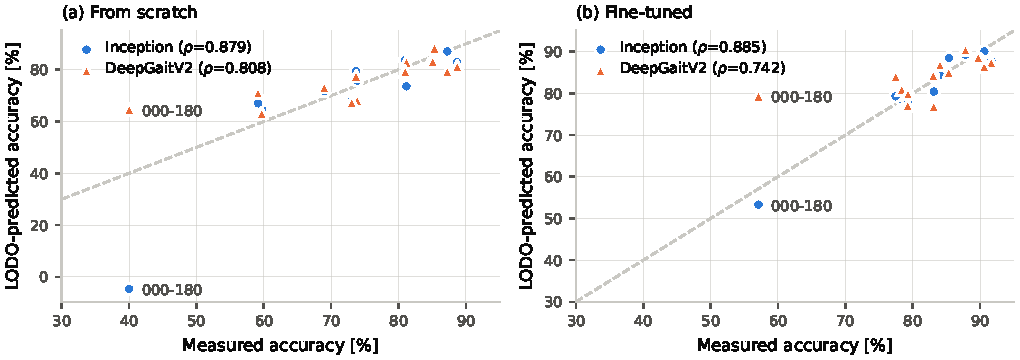
\includegraphics[width=13.5cm,bb=0 0 489.6 172.8]{fig_pred_vs_true_X2_2panel_20260907.pdf}
\caption{実測精度と LODO 予測精度の関係（Inception 6 変数と DeepGaitV2 6 変数）．(a) スクラッチ学習，(b) ファインチューニング後．破線は $y=x$．000-180 はスクラッチ学習で外挿となり，Inception 6 変数の予測値は負になる．}
\label{fig:pred}
\end{figure*}

\subsection{データセット優劣判定}
%% 優劣判定の表（tables/table_pairwise.tex）はページ都合で本文に圧縮（9/10）。戻す場合はこの節末に %% 自動生成: make_tables_20260915.py（手で編集しない）
\begin{table}[tb]
\caption{データセット優劣判定の性能（156 順序対，leave-one-pair-out，$\tau=0.05$）．M-F1 は Macro-F1．}
\label{tab:pairwise}
\begin{center}
\begin{tabular}{l|cc|cc}
\Hline
 & \multicolumn{2}{c|}{スクラッチ} & \multicolumn{2}{c}{ファインチューニング} \\
特徴空間 & Acc & M-F1 & Acc & M-F1 \\
\hline
Inception（6 変数） & 0.859 & 0.847 & 0.795 & 0.800 \\
DINOv2（6 変数） & 0.769 & 0.756 & 0.756 & 0.763 \\
Inception+DINOv2（11 変数） & 0.846 & 0.835 & 0.795 & 0.801 \\
DeepGaitV2（6 変数） & 0.859 & 0.847 & 0.731 & 0.737 \\
\Hline
\end{tabular}
\end{center}
\end{table}
 を追加
優劣判定では，スクラッチ学習で Inception 6 変数と DeepGaitV2 6 変数が Acc 0.859，Macro-F1 0.847 で並び，ファインチューニング後では Inception 6 変数と 11 変数がいずれも Acc 0.795（Macro-F1 0.800，0.801．11 変数の並べ替え検定 $p=0.010$），DINOv2 6 変数が 0.756，DeepGaitV2 6 変数が 0.731 で最も低かった．最多クラスを常に予測した場合の Acc（スクラッチ学習 0.385，ファインチューニング後 0.397）はいずれの特徴空間も大きく上回る．ファインチューニング後は同等の対が多く（62/156 対 36/156），Acc は予測対象間で比較しない．

\subsection{条件別の予測性能}
表\ref{tab:condition}に，NM/BG/CL 各条件の Rank-1 を目的変数とした LODO 予測の性能を，汎用画像特徴（11 変数）と歩容特化特徴（6 変数）について示す．条件別の目的変数は 4.\,1 節の精度の構成要素であり，主結果とは独立でない探索的解析で，特徴空間間の差の検定は行っていない．NM と BG では両特徴空間の $\rho$ の差は 0.17 以下で一貫した優劣はない．これに対し CL では歩容特化特徴がスクラッチ学習 0.956，ファインチューニング後 0.896 と両予測対象で高く，汎用画像特徴の 0.665，0.511 を上回った．歩容特化特徴では CL で 3 条件中最も高い順位相関が得られたのに対し，汎用画像特徴では CL の順位相関が最も低く，得意な条件が特徴空間で異なる傾向を観測した．なお CL の MAE は両特徴空間とも 3 条件中で最大であったが，条件ごとに目的変数の分布が異なるため MAE の大小だけで予測の難しさは判断しない．
%% 自動生成: make_tables_20260915.py（手で編集しない）
\begin{table}[tb]
\caption{条件別（NM/BG/CL Rank-1）の学習前予測性能．汎用は Inception+DINOv2（11 変数），歩容特化は DeepGaitV2（6 変数）．MAE の単位は pt．13 サブセットの記述統計で検定は行っていない．}
\label{tab:condition}
\begin{center}
\begin{tabular}{ll|cc|cc}
\Hline
 & & \multicolumn{2}{c|}{汎用} & \multicolumn{2}{c}{歩容特化} \\
予測対象 & 条件 & $\rho$ & MAE & $\rho$ & MAE \\
\hline
スクラッチ & NM & 0.758 & 9.21 & 0.868 & 7.41 \\
 & BG & 0.879 & 8.82 & 0.835 & 4.48 \\
 & CL & 0.621 & 22.17 & 0.956 & 7.66 \\
\hline
ファインチューニング & NM & 0.824 & 3.21 & 0.753 & 4.41 \\
 & BG & 0.885 & 2.95 & 0.819 & 3.67 \\
 & CL & 0.533 & 18.81 & 0.896 & 6.26 \\
\Hline
\end{tabular}
\end{center}
\end{table}


\subsection{回帰係数}
%% 係数表（tables/table_coef_ft.tex）はページ都合で本文に圧縮（9/10）。戻す場合はこの節末に %% 自動生成: make_tables_20260915.py（手で編集しない）
\begin{table}[tb]
\caption{ファインチューニング後精度に対する標準化リッジ係数（LODO 13 回の平均，pt/SD）．}
\label{tab:coef}
\begin{center}
\begin{tabular}{l|rr}
\Hline
指標 & Inception & DeepGaitV2 \\
\hline
$\log P$（人数） & $+1.92$ & $+3.02$ \\
MSD（平均クラス内分散） & $+1.98$ & $-0.67$ \\
1NN & $+1.50$ & $+0.76$ \\
kNN ($k=5$) & $+2.04$ & $+2.93$ \\
pairFID（平均クラス間距離） & $-1.88$ & $+0.10$ \\
FID$_{\mathrm{tt}}$（Train-Test 分布距離） & $-3.60$ & $-5.17$ \\
\Hline
\end{tabular}
\end{center}
\end{table}
 を追加
ファインチューニング後精度に対する標準化リッジ係数（LODO 13 回の平均，pt/SD）は，FID$_{\mathrm{tt}}$ が Inception 6 変数で $-3.60$，DeepGaitV2 6 変数で $-5.17$ と両特徴空間で負であり，6 変数中で絶対値が最大であった．スクラッチ学習でも FID$_{\mathrm{tt}}$ の係数は負（InceptionV3 $-4.49$，DeepGaitV2 $-9.74$）で，4 通りすべてで符号が一致した．ただし 11 変数では $\log P$（$+1.91$），InceptionV3 の kNN（$+1.76$），MSD（$+1.46$），1NN（$+1.40$）の方が絶対値で FID$_{\mathrm{tt}}$（$-1.29$）より大きく，「FID$_{\mathrm{tt}}$ が最重要」は 6 変数の場合に限られる．

%% =====================================================================
\section{考察}
\subsection{テスト分布からの距離}
FID$_{\mathrm{tt}}$ の係数が 4 通りすべてで負であることは，他の指標を統制したうえでもテスト分布から遠い学習データほど到達精度が低いという関係が，今回比較した特徴空間のいずれでも，事前学習の有無に依らず保たれていることと整合する．生の順位相関でも FID$_{\mathrm{tt}}$ は NM，CL の条件別の精度と負であった（InceptionV3 $-0.49$〜$-0.68$，DeepGaitV2 $-0.58$〜$-0.84$）．ファインチューニング後に係数の絶対値が減少したこと（InceptionV3 $-4.49\to-3.60$，DeepGaitV2 $-9.74\to-5.17$）は，事前学習が分布差の影響を緩和した可能性と整合するが，目的変数の範囲が圧縮された効果も含まれるため，係数の差のみから断定はできない．
なお歩容特化特徴はファインチューニングの初期値と同一モデルの特徴空間であるが，今回の 13 サブセットではファインチューニング後精度の順位予測で汎用画像特徴を上回らなかった（0.742 と 0.890．目的変数の定義にも依存する，7 章）．

\subsection{数値予測の限界}
順位相関が高くても，精度の絶対値は外れうる．視野角を $0^\circ$ と $180^\circ$ に制限した 000-180 では，汎用画像特徴（11 変数）のスクラッチ学習精度の LODO 予測値が $-28.7\%$（実測 40.0\%，誤差 $-68.7$\,pt）と負になり，Inception 6 変数でも $-4.6\%$ であった（図\ref{fig:pred}(a)）．DeepGaitV2 6 変数では逆に 64.6\%（誤差 $+24.6$\,pt）であった．汎用画像特徴（11 変数）ではこの 1 サブセットが絶対誤差の総和の約 55\%（ファインチューニング後は約 56\%）を占め，残る 12 サブセットの MAE はスクラッチ学習 4.62\,pt（全体 9.55\,pt），ファインチューニング後 1.62\,pt（同 3.39\,pt）である．原因の一つとして，LODO では 000-180 を除いた 12 サブセットで標準化と回帰を行うため，000-180 の FID$_{\mathrm{tt}}$（InceptionV3 で 33.1，他のサブセットは 9.9 以下）が学習範囲の外側に外れ，線形モデルの外挿となることが考えられる．一方，汎用画像特徴 11 変数では 000-180 は実測・予測とも最下位で順位相関には寄与する側であり，評価点から除いた 12 サブセットの $\rho$ も 11 変数で 0.839（スクラッチ学習），0.860（ファインチューニング後），DeepGaitV2 6 変数で 0.769，0.734 と高い（残る 12 点の予測モデルの学習には 000-180 が含まれる）．
なお 000-180 はファインチューニング後精度（57.11\%）が zero-shot 精度（70.83\%）を下回った唯一のサブセットである（同じく視野角 2 点の 000-090，090-180 は上回った）．1 サブセットの観測であり断定はできない．本稿の主張は順位予測の有効性であり，数値予測は外挿域で破綻することを併せて報告する．

%% =====================================================================
\section{まとめと今後の展望}
本稿は，深層特徴空間上のデータ特性指標から認証精度を学習前に予測する中村らの枠組みを，予測対象（ファインチューニング後精度）と特徴空間（歩容特化特徴）の両方向に拡張した．CASIA-B の 13 サブセットの LODO 評価では 4 通りすべてで順位相関は $\rho=0.74$〜$0.89$ であり，汎用画像特徴のみでもファインチューニング後精度との順位相関は $\rho=0.83$〜$0.89$ であった．今回の 13 サブセットでは CL 条件で歩容特化特徴の順位相関が高く，一方で視野角を極端に制限したサブセットでは数値予測が大きく外れ，順位予測と数値予測は分けて評価する必要がある．

本稿の結論は次の範囲に限られる．13 サブセットは同一の CASIA-B から構成した独立でない標本であり，FID$_{\mathrm{tt}}$ の参照集合と評価集合も共通である．回帰の構築には他サブセットの実測精度を要するため，未知の評価環境に学習データだけから適用できることを示したものではない．事前学習元・認証モデル・入力は 1 種類ずつで，ファインチューニングは単一シードで 1 回ずつ行い，シード間の変動は評価していない．スクラッチ学習精度とファインチューニング後精度の順位相関は 0.973 と高く，ファインチューニング後の順位相関はファインチューニングに固有の変化を捉えたことを意味しない．反復数と学習率も異なるため $\Delta$ を事前学習のみの効果とは断定できず，$\Delta$ と DeepGaitV2 の FID$_{\mathrm{tt}}$ の偏順位相関（スクラッチ学習精度を統制）も $-0.200$（$p=0.534$，両側 $t$ 近似）で有意でなかったため，$\Delta$ の予測は主張に含めない．特徴空間間の $\rho$ の差の検定は行っておらず優劣を断定しない．実際，目的変数を NM/BG/CL の単純平均に変えると，11 変数の $\rho$ は 0.879 とほぼ不変だが 6 変数ではファインチューニング後の大小が入れ替わる（Inception 0.885 から 0.786，DeepGaitV2 0.742 から 0.791）．また InceptionV3 と DINOv2 の指標の一部は中村らの計測値を引き継いでおり（4.\,4 節），MSD を式\eqref{eq:MSD}のとおり人物ごとに計算して集計を揃えることも行っていない．

今後の課題は二つある．第一に外部検証である．汎用画像特徴で順位相関が得られるなら，歩容以外のタスクや別の事前学習元にも同じ手順を持ち込める可能性がある．一方，認証対象に固有の変動（歩容では服装）が主要な難しさになる条件では歩容特化特徴の方が良い可能性があり，服装変動を含まないデータセット（OU-MVLP\cite{Takemura_OUMVLP}）と含むデータセット（GREW\cite{Zhu_GREW}，Gait3D\cite{Zheng_Gait3D}）で結果が分かれるかを検証したい．第二に，外挿域の検出である．FID$_{\mathrm{tt}}$ が既知のサブセットの範囲を大きく超える場合に数値予測を保留する規準を設けたい．

%% TODO(決定B-3): 謝辞（中村論文は JSPS 科研費 25K03120）
%% \ack はコマンド（環境ではない）。文を決めたら次の1行のコメントを外す。\ack と謝辞文の間に空行を入れない（readme.tex）
%% \ack 本研究の一部はJSPS科研費 XXXXXXXX の助成を受けたものである．

\bibliographystyle{sieicej}
\bibliography{Myref_add}% Myref_add.bib（yokou/ からコピー＋5件追加）。Overleaf に Myref.bib 本体があるなら統合する

\end{document}
